% !TeX program = lualatex
% !TeX encoding = utf8
% !TeX spellcheck = uk_UA
% !BIB program = bibler

\documentclass[onlytextwidth]{beamer}
\usetheme{Electromagnetism}

\usepackage{Electromagnetism}
\usepackage{circuitikz}
\usepackage{pgfplots}
\pgfplotsset{compat=1.17}
\usetikzlibrary{arrows.meta,calc}
\hypersetup{
  colorlinks=true,
  linkcolor=cyan,  % Цвет для внутренних ссылок
  urlcolor=red,    % Цвет для URL
  citecolor=blue   % Цвет для библиографических ссылок
}




%============================================================================
\title[Лекції електрики та магнетизму]{\huge\bfseries Довгі лінії. \\ Телеграфні рівняння}
\subtitle{Лекції з електрики та магнетизму}
\author{Пономаренко С. М.}
\date{}
%============================================================================
\graphicspath{{pictures/}}
\begin{document}


\begin{frame}[plain]
	\maketitle
\end{frame}

% ============================== Слайд ## ===================================
\begin{frame}{Зміст лекції}{}
	\tableofcontents
\end{frame}
% ===========================================================================

%% --------------------------------------------------------
\section{Від зосереджених елементів до розподілених}
%% --------------------------------------------------------

% ============================== Слайд ## ===================================
\begin{frame}{Від зосереджених елементів до розподілених}{}
	\begin{block}{}\justifying
		Якщо довжина кола $l$ вже не набагато менша за довжину хвилі $\lambda=cT$ (магістральна ЛЕП, кабель зв'язку, доріжка на платі), напруга й струм у різних точках лінії зсунуті за фазою --- скінченний набір $R,L,C$ більше не описує коло.
	\end{block}
	\begin{exampleblock}{}\justifying\small
		Трансатлантичний телеграфний кабель (1858 р.) передавав лише кілька слів на хвилину: кабель довжиною в тисячі кілометрів уже не був квазістаціонарним. Теорію розробили В.~Томсон (лорд Кельвін) та О.~Гевісайд.
	\end{exampleblock}
	\begin{block}{}\justifying
		Лінію описують \alert{погонними параметрами} (на одиницю довжини):
		\begin{equation*}
			R_0\ \left[\tfrac{\text{Ом}}{\text{м}}\right], \quad
			L_0\ \left[\tfrac{\text{Гн}}{\text{м}}\right], \quad
			G_0\ \left[\tfrac{\text{См}}{\text{м}}\right], \quad
			C_0\ \left[\tfrac{\text{Ф}}{\text{м}}\right].
		\end{equation*}
		$G_0$ --- провідність витоку через недосконалість ізоляції ($G_0=0$ для ідеальної лінії).
	\end{block}
\end{frame}
% ===========================================================================

%% --------------------------------------------------------
\section{Телеграфні рівняння}
%% --------------------------------------------------------

% ============================== Слайд ## ===================================
\begin{frame}{Виведення телеграфних рівнянь}{}
	\begin{columns}
		\begin{column}{0.6\linewidth}\centering
			\begin{circuitikz}[european resistors, scale=0.75]
				\draw (0,0) to[short, o-] (0.5,0)
				      to[R, l=$R_0\,dz$] (2.5,0)
				      to[L, l=$L_0\,dz$] (4.5,0)
				      to[short, -o] (5.5,0);
				\draw (0,-2) to[short, o-] (5.5,-2);
				\draw (4.5,0) to[C, l_=$C_0\,dz$, *-*] (4.5,-2);
				\draw (3.0,0) to[R, l_=$G_0\,dz$, *-*] (3.0,-2);
				\draw (0,0) to[open, v^=$u$] (0,-2);
				\draw (5.5,0) to[open, v^=$u{+}du$] (5.5,-2);
			\end{circuitikz}
		\end{column}
		\begin{column}{0.4\linewidth}\justifying\small
			Елемент лінії довжиною $dz$. Друге правило Кірхгофа для верхньої гілки і перше правило для вузла на виході, у границі $dz\to0$, дають:
		\end{column}
	\end{columns}
	\begin{block}{}\justifying
		\alert{Телеграфні рівняння} (часова форма):
		\begin{equation*}
			\tcbhighmath{
				-\frac{\partial u}{\partial z} = R_0 i + L_0\frac{\partial i}{\partial t}, \qquad
				-\frac{\partial i}{\partial z} = G_0 u + C_0\frac{\partial u}{\partial t}.
			}
		\end{equation*}
	\end{block}
	\begin{exampleblock}{}\justifying\small
		По суті --- закон Ома і правила Кірхгофа для нескінченно малого відрізка лінії; при $L_0=C_0=0$ зводяться до звичайного закону Ома для розподіленого опору.
	\end{exampleblock}
\end{frame}
% ===========================================================================

%% --------------------------------------------------------
\section{Гармонічний режим. Хвильове рівняння}
%% --------------------------------------------------------

% ============================== Слайд ## ===================================
\begin{frame}{Хвильове рівняння. Стала поширення}{}
	\begin{block}{}\justifying
		Для гармонічного сигналу ($u,i\propto e^{i\omega t}$, комплексні амплітуди $V(z)$, $I(z)$) телеграфні рівняння набирають вигляду
		\begin{equation*}
			-\frac{dV}{dz} = (R_0+i\omega L_0)I, \qquad
			-\frac{dI}{dz} = (G_0+i\omega C_0)V.
		\end{equation*}
		Виключаючи $I$, отримуємо рівняння Гельмгольца $d^2V/dz^2=\gamma^2V$, де
		\begin{equation*}
			\tcbhighmath{
				\gamma = \sqrt{(R_0+i\omega L_0)(G_0+i\omega C_0)} = \alpha + i\beta
			}
		\end{equation*}
		--- \alert{стала поширення} ($\alpha$ --- стала затухання, $\beta$ --- фазова стала).
	\end{block}
	\begin{exampleblock}{}\justifying
		Загальний розв'язок:
		\begin{equation*}
			\tcbhighmath{
				V(z) = V^+e^{-\gamma z} + V^-e^{+\gamma z}.
			}
		\end{equation*}
		$V^+$ --- хвиля до навантаження ($+z$), $V^-$ --- відбита хвиля ($-z$); $\lambda=2\pi/\beta$, $v_{\text{ф}}=\omega/\beta$.
	\end{exampleblock}
\end{frame}
% ===========================================================================

% ============================== Слайд ## ===================================
\begin{frame}{Хвильовий опір лінії}{}
	\begin{block}{}\justifying
		З рівнянь для $V(z)$ і $I(z)$:
		\begin{equation*}
			I(z) = \frac1{Z_{\text{хв}}}\left(V^+e^{-\gamma z} - V^-e^{+\gamma z}\right), \qquad
			\tcbhighmath{
				Z_{\text{хв}} = \frac{R_0+i\omega L_0}{\gamma} = \sqrt{\frac{R_0+i\omega L_0}{G_0+i\omega C_0}}.
			}
		\end{equation*}
	\end{block}
	\begin{exampleblock}{}\justifying\small
		$Z_{\text{хв}}$ --- не опір ділянки, а відношення $V/I$ саме в \alert{біжучій} хвилі. Якщо навантаження $Z_\text{н}=Z_{\text{хв}}$, відбитої хвилі немає ($V^-=0$) --- узгодження навантаження з $Z_{\text{хв}}$ (напр., $50$ Ом) --- ключова задача НВЧ-техніки.
	\end{exampleblock}
\end{frame}
% ===========================================================================

%% --------------------------------------------------------
\section{Лінія без втрат}
%% --------------------------------------------------------

% ============================== Слайд ## ===================================
\begin{frame}{Лінія без втрат}{}
	\begin{block}{}\justifying
		При $R_0=G_0=0$ стала поширення чисто уявна:
		\begin{equation*}
			\tcbhighmath{
				\gamma = i\beta, \qquad \beta = \omega\sqrt{L_0C_0}, \qquad \alpha=0.
			}
		\end{equation*}
		Хвиля поширюється без затухання; фазова швидкість не залежить від частоти:
		\begin{equation*}
			v_{\text{ф}} = \frac1{\sqrt{L_0C_0}}, \qquad \lambda = \frac{2\pi}{\omega\sqrt{L_0C_0}}.
		\end{equation*}
	\end{block}
	\begin{block}{}\justifying
		Хвильовий опір стає дійсним:
		\begin{equation*}
			\tcbhighmath{
				Z_{\text{хв}} = \sqrt{\frac{L_0}{C_0}}.
			}
		\end{equation*}
		Якщо відбитої хвилі немає, напруга й струм у кожній точці лінії --- у фазі.
	\end{block}
\end{frame}
% ===========================================================================

% ============================== Слайд ## ===================================
\begin{frame}{Стояча хвиля}{}
	\begin{columns}
		\begin{column}{0.46\linewidth}\justifying\small
			За наявності відбитої хвилі:
			\begin{equation*}
				u(z,t) = |V^+|\cos(\omega t-\beta z) + |V^-|\cos(\omega t+\beta z+\pi).
			\end{equation*}
			Інтерференція дає \alert{стоячу хвилю} з вузлами й пучностями. Коефіцієнт стоячої хвилі:
			\begin{equation*}
				\tcbhighmath{
					\text{КСХ} = \frac{1+|V^-/V^+|}{1-|V^-/V^+|}.
				}
			\end{equation*}
		\end{column}
		\begin{column}{0.54\linewidth}\centering
			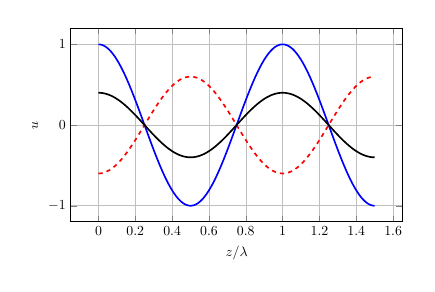
\begin{tikzpicture}[scale=0.5]
				\begin{axis}[
						width=10cm, height=6.5cm, xlabel={$z/\lambda$}, ylabel={$u$},
						domain=0:1.5, samples=300, grid=both, thick,
						every axis plot/.append style={very thick}
					]
					\addplot[blue] {cos(deg(2*pi*x))};
					\addplot[red, dashed] {0.6*cos(deg(2*pi*x)+180)};
					\addplot[black] {cos(deg(2*pi*x)) + 0.6*cos(deg(2*pi*x)+180)};
				\end{axis}
			\end{tikzpicture}
		\end{column}
	\end{columns}
\end{frame}
% ===========================================================================

% ============================== Слайд ## ===================================
\begin{frame}{Дисперсія сигналу}{}
	\begin{exampleblock}{}\justifying\small
		У реальній лінії $v_{\text{ф}}$ залежить від частоти --- спектральні складові біжать з різною швидкістю, і імпульс \alert{«розмазується»}. Саме це мучило перші трансатлантичні кабелі. Гевісайд (1890-ті) показав: спотворень немає, якщо
		\begin{equation*}
			\tcbhighmath{
				\frac{R_0}{L_0} = \frac{G_0}{C_0}
			}
		\qquad\text{\alert{лінія без спотворень}}.
		\end{equation*}
	\end{exampleblock}
	\begin{center}
		\begin{tikzpicture}[scale=0.5]
			\begin{axis}[
					width=11cm, height=6cm, xlabel={$t$, ум.\,од.}, ylabel={$u(t)$},
					domain=-3:18, samples=300, grid=both, thick,
					every axis plot/.append style={very thick},
					legend pos=north east, legend style={font=\tiny}
				]
				\addplot[black] {exp(-x^2)};
%				\addlegendentry{$z=0$}
				\addplot[blue] {0.75*exp(-(x-5)^2/2.25)};
%				\addlegendentry{$z{=}100$ км}
				\addplot[red, dashed] {0.4*exp(-(x-12)^2/9)};
%				\addlegendentry{$z{=}300$ км}
				\addplot[orange, dotted] {0.18*exp(-(x-15)^2/25)};
%				\addlegendentry{$z{=}1000$ км}
			\end{axis}
		\end{tikzpicture}
	\end{center}
\end{frame}
% ===========================================================================

%% --------------------------------------------------------
\section{Польова картина. Зв'язок з рівняннями Максвелла}
%% --------------------------------------------------------

% ============================== Слайд ## ===================================
\begin{frame}{Поле в довгій лінії. ТЕМ-хвиля}{}
	\begin{columns}
		\begin{column}{0.46\linewidth}\justifying\small
			Зв'язок поля з величинами кола:
			\begin{equation*}
				u = \int_1^2 \Efield\cdot d\vect r, \qquad
				i = \oint_{C_h} \Hfield\cdot d\vect r.
			\end{equation*}
			$\Efield$ (поперечне, від різниці потенціалів) і $\Hfield$ (поперечне, від струму) обидва $\perp z$ --- \alert{поперечна електромагнітна хвиля} (ТЕМ). Вектор Пойнтінга $\vect S=\frac{c}{4\pi}[\Efield\times\Hfield]$ напрямлений уздовж $z$.
		\end{column}
		\begin{column}{0.54\linewidth}\centering
			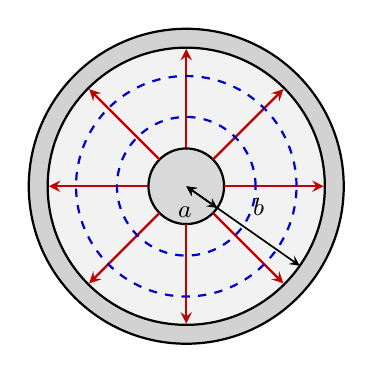
\begin{tikzpicture}[scale=0.8, >=latex]
				\tikzset{
					Eline/.style={->, >=stealth, red!75!black, thick},
					Hline/.style={blue!80!black, thick, dashed}
				}
				\fill[gray!10] (0,0) circle (2.2);
				\fill[gray!30] (0,0) circle (0.6);
				\draw[thick] (0,0) circle (0.6);
				\fill[gray!35, even odd rule] (0,0) circle (2.5) (0,0) circle (2.2);
				\draw[thick] (0,0) circle (2.2);
				\draw[thick] (0,0) circle (2.5);
				\foreach \angle in {0, 45, 90, 135, 180, 225, 270, 315} {
						\draw[Eline] (\angle:0.6) -- (\angle:2.18);
					}
				\node[red!75!black, above right] at (50:1.4) {$\Efield$};
				\foreach \r in {1.1, 1.75} {
						\draw[Hline] (0,0) circle (\r);
					}
				\node[blue!80!black, above left] at (140:1.1) {$\Hfield$};
				\draw[<->, >=stealth, semithick] (0,0) -- (-35:0.6) node[midway, below left] {\small $a$};
				\draw[<->, >=stealth, semithick] (0,0) -- (-35:2.2) node[midway, above right] {\small $b$};
			\end{tikzpicture}
		\end{column}
	\end{columns}
\end{frame}
% ===========================================================================

% ============================== Слайд ## ===================================
\begin{frame}{Універсальне співвідношення $L_0C_0$}{}
	\begin{exampleblock}{}\justifying\small
		Провідники самі не «проштовхують» енергію --- вони \alert{напрямляють} електромагнітну хвилю (лінія --- окремий випадок хвилеводу для ТЕМ-хвилі), задаючи граничні умови для $\Efield$ і $\Hfield$.
	\end{exampleblock}
	\begin{block}{}\justifying
		Оскільки структура поля в перерізі --- електро-/магнітостатична, з рівнянь Максвелла для будь-якої лінії з двох провідників:
		\begin{equation*}
			\tcbhighmath{
				L_0C_0 = \varepsilon_0\varepsilon\,\mu_0\mu.
			}
		\end{equation*}
		Звідси фазова швидкість не залежить від геометрії провідників:
		\begin{equation*}
			\tcbhighmath{
				v_{\text{ф}} = \frac1{\sqrt{L_0C_0}} = \frac{c}{\sqrt{\varepsilon\mu}}.
			}
		\end{equation*}
		Сигнал у лінії поширюється зі швидкістю світла в діелектрику лінії.
	\end{block}
\end{frame}
% ===========================================================================

% ============================== Слайд ## ===================================
\begin{frame}{Приклад: коаксіальний кабель}{}
	\begin{block}{}\justifying
		За теоремою Гаусса і законом Ампера для жили радіусом $a$ й екрана радіусом $b$:
		\begin{equation*}
			C_0 = \frac{2\pi\varepsilon_0\varepsilon}{\ln(b/a)}, \qquad
			L_0 = \frac{\mu_0\mu}{2\pi}\ln\!\left(\frac ba\right), \qquad
			\tcbhighmath{
				Z_{\text{хв}} = \frac{\eta}{2\pi}\ln\!\left(\frac ba\right),
			}
		\end{equation*}
		де $\eta=\sqrt{\mu_0\mu/\varepsilon_0\varepsilon}$ --- хвильовий опір діелектрика ($\eta_0\approx377$ Ом для вакууму).
	\end{block}
	\begin{exampleblock}{}\justifying\small
		При $a=0.5$ мм, $b=2.0$ мм, $\varepsilon=2.25$ ($\mu=\mu_0$): $\ln(b/a)\approx1.386$, звідки
		\begin{equation*}
			C_0\approx90.3\ \text{пФ/м}, \quad L_0\approx277\ \text{нГн/м}, \quad
			Z_{\text{хв}}\approx55.4\ \text{Ом}, \quad v_{\text{ф}}=\frac c{1.5}=2\times10^8\ \tfrac{\text{м}}{\text{с}}.
		\end{equation*}
	\end{exampleblock}
\end{frame}
% ===========================================================================

% ============================== Слайд ## ===================================
\begin{frame}{Підсумки}{}
\begin{tblr}{
colspec={Q[c,l]Q[mode=dmath]}
}
Телеграфні рівняння & -\partial_z u = R_0 i + L_0\partial_t i,\quad -\partial_z i = G_0 u + C_0\partial_t u \\
Стала поширення & \gamma=\sqrt{(R_0+i\omega L_0)(G_0+i\omega C_0)} = \alpha+i\beta \\
Розв'язок для напруги & V(z) = V^+e^{-\gamma z} + V^-e^{+\gamma z} \\
Хвильовий опір & Z_{\text{хв}} = \sqrt{\dfrac{R_0+i\omega L_0}{G_0+i\omega C_0}} \\
Лінія без втрат & \gamma=i\beta,\ \beta=\omega\sqrt{L_0C_0},\ Z_{\text{хв}}=\sqrt{L_0/C_0} \\
Фазова швидкість & v_{\text{ф}} = \omega/\beta = 1/\sqrt{L_0C_0} \\
Лінія без спотворень & R_0/L_0 = G_0/C_0 \\
Універсальне співвідношення & L_0C_0 = \varepsilon_0\varepsilon\mu_0\mu \\
Фазова швидкість (польовий підхід) & v_{\text{ф}} = c/\sqrt{\varepsilon\mu} \\
Коаксіальний кабель & Z_{\text{хв}} = \dfrac{\eta}{2\pi}\ln(b/a)
\end{tblr}
\end{frame}
% ===========================================================================

\end{document}